\documentclass[10pt,twocolumn,letterpaper]{article}

\usepackage{cvpr}
\usepackage{times}
\usepackage{epsfig}
\usepackage{graphicx}
\usepackage{amsmath}
\usepackage{amssymb}
\usepackage{gensymb}

% Include other packages here, before hyperref.

% If you comment hyperref and then uncomment it, you should delete
% egpaper.aux before re-running latex.  (Or just hit 'q' on the first latex
% run, let it finish, and you should be clear).
\usepackage[pagebackref=true,breaklinks=true,letterpaper=true,colorlinks,bookmarks=false]{hyperref}

% \cvprfinalcopy % *** Uncomment this line for the final submission

\def\cvprPaperID{****} % *** Enter the CVPR Paper ID here
\def\httilde{\mbox{\tt\raisebox{-.5ex}{\symbol{126}}}}

% Pages are numbered in submission mode, and unnumbered in camera-ready
\ifcvprfinal\pagestyle{empty}\fi
\begin{document}

%%%%%%%%% TITLE
\title{Interaction-aware Attention-measurable Visual Navigation in Crowds}

\author{First Author\\
Institution1\\
Institution1 address\\
{\tt\small firstauthor@i1.org}
% For a paper whose authors are all at the same institution,
% omit the following lines up until the closing ``}''.
% Additional authors and addresses can be added with ``\and'',
% just like the second author.
% To save space, use either the email address or home page, not both
\and
Second Author\\
Institution2\\
First line of institution2 address\\
{\tt\small secondauthor@i2.org}
}

\maketitle
%\thispagestyle{empty}

%%%%%%%%% ABSTRACT
\begin{abstract}
   Recent works have shown the strong capacity of deep neural networks in learning a navigation policy from visual input. Interpreting the powerful end-to-end approach, however, is generally difficult, raising significant concerns regarding its safety for autonomous navigation in human crowds. In this work, we present a visual navigation model that is interpretable by not only qualitative visualization but also quantitative measurements. 


   \vspace{3cm}
\end{abstract}

%%%%%%%%% BODY TEXT


%%%%%%%%%%%%%%%%%%%%%%%%%%%%%%%%%%%%%%%%%%%%%%%%%%%%%%%%%%%%%%%%%%%%%%%%%%
%                 Introduction
%%%%%%%%%%%%%%%%%%%%%%%%%%%%%%%%%%%%%%%%%%%%%%%%%%%%%%%%%%%%%%%%%%%%%%%%%%

\section{Introduction}

Autonomous navigation is an essential skill that mobile robots and self-driving vehicles need to acquire. Although great progress has been made, building a navigation algorithm towards human-level intelligence is challenging \cite{urmson_autonomous_2009, levinson_towards_2011, sunderhauf_limits_2018}. In particular, navigation in complex scenarios calls for a strong ability in scene understanding \cite{li_towards_2009, cordts_cityscapes_2016}, relational reasoning \cite{santoro_simple_2017}, behavior prediction \cite{alahi_social_2016} and motion planning \cite{latombe_robot_2012}, most of which can be hardly described by human-designed functions. To address these challenges, deep neural networks have become a central and promising tool for developing navigation policies \cite{muller_off-road_2006,bojarski_end_2016, shalev-shwartz_safe_2016}. 

Neural network models, despite their superior modelling capacities, often suffer from weak interpretability \cite{zhang_visual_2018}, which is of significant importance when autonomous vehicles come to safety-critical environments. A large body of work tries to blend the capability of neural networks and the interpretability of hand-engineered functions by constructing a sequential pipeline for navigation systems \cite{urmson_autonomous_2009}, comprising of various components including detection \cite{he_mask_2017}, tracking \cite{bertinetto_fully-convolutional_2016, nam_learning_2016}, mapping \cite{zhang_neural_2017}, and control \cite{gupta_cognitive_2017, chen_crowd-robot_2018}. On one hand, this sequential pipeline provides us a form of interpretability through an access to the outputs of intermediate stages; on the other hand, it fails to capture the inherent dependencies between components and waste unnecessary compuations on objects trivial for planning, which degrades navigation performance. 


\begin{figure}[t]
  \centering
  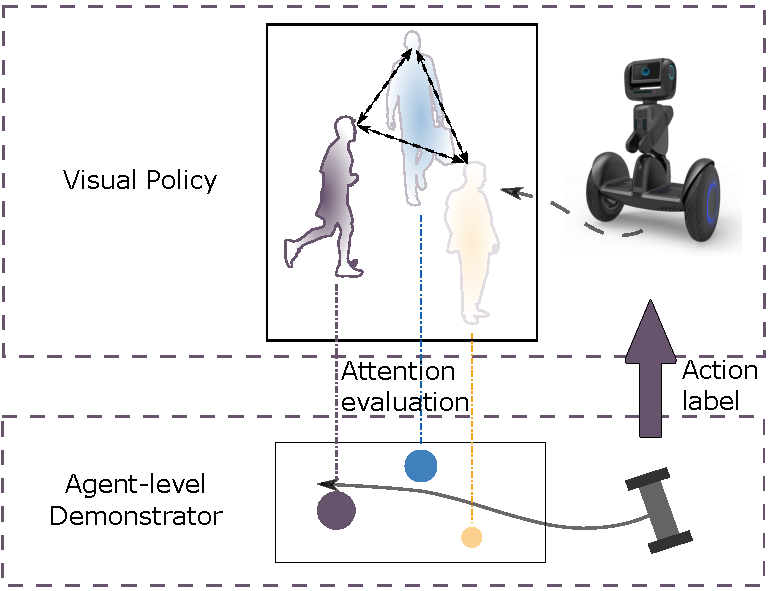
\includegraphics[width=1.0\linewidth]{figures/pull.pdf}
  \caption{Visual attention allows end-to-end policy to focus on certain image regions and make interpretable decisions for navigation in dynamic crowds. However, the correctness of a model's attention is hard to measure. We propose a method to quantify attention consistency between end-to-end learners (top) and an attention-driven demonstrator (bottom) across domains, paving the way for understanding navigation causality in complex scenes.}
\end{figure}

In contrast to hand-crafted pipelines, some end-to-end approaches use visualization techniques to enhance its interpretability. \cite{simonyan_deep_2013, selvaraju_grad-cam:_2016} propose to compute a saliency map specific to a given image and output, which has been applied to navigation tasks \cite{bojarski_explaining_2017,chi_deep_2017}. More recently, \cite{kim_interpretable_2017} presents an interpretable policy learning method that combines saliency visualization with an attention mechanism. These interpretation methods, however, are subject to qualitative interpretation, prevent us from quantifying the degree that a neural policy can capture the "real" effect. 

The primary goal of this work is to develop an end-to-end and quantitatively interpretable neural network policy for autonomous navigation in highly dynamic and densely populated spaces, which is by itself a very challenging problem due to complex crowd-robot interactions \cite{chen_crowd-robot_2018}. To this end, we propose a goal driven dual attention model that directly maps raw depth image to control actions. Leveraging on recent progress in non-local neural networks \cite{wang_non-local_2017}, our model learns a feature representation that can effectively take both the goal information and agents relationship into account. We train the proposed end-to-end policy using trajectories recorded from a demonstrator in an imitation learning framework and show in empirical experiments that it outperforms standard CNN policy in terms of task accomplishments. 

To quantitatively examine the proposed attention mechanism for crowd navigation, we design an simulation environment that allows us to measure the consistency between the attention from a learned model and that from a demonstrator, inspired by the attention measures in image domains \cite{das_human_2016, liu_neural_2016}. Specifically, we build a pipeline-based attention-driven demonstrator with agent-level 2d information as input. This demonstrator can provide attention information along with action labels, offering a comparable attention metric for learners. By measuring statistical distances between attentions across domains, we show that our proposed dual attention policy can accurately infer the inherent attention of the simulated demonstrator. The high consistency of attended regions indicates a strong potential of the proposed method in learning attentions of human drivers that is usually hard to reveal, suggesting a promising direction towards the understanding of causality for navigation in complex scenes. The developed simulation environment for attention evaluation will be released to the public soon. 

% %%%%%%%%% BODY TEXT
% \section{Introduction}

% The recent development of deep learning has boosted the performance of many perceptual learning tasks e.g. classification, object detection and etc, while bringing the deep learning powered perceptual ability to real-world tasks, e.g. robot navigation \cite{mirowski_learning_2018, zhu_target-driven_2016}, autonomous driving remains challenging. There are two common approach to tackle that problem: end-to-end approach and layered stack. End-to-end methods \cite{bojarski_end_2016} map raw sensor input to actions, which benefits from rich visual information but also often lacks interpretability and reliability. A layered stack breaks a task into several steps, e.g. detection, prediction and planning \cite{everett_motion_2018}, where the intermediate results are interpretable while different stacks don't benefit from end-to-end learning.

% % [shall we talk about the problem in this specific scenario?]
% % Navigation in crowded space with visual input is very challenging due to the hidden intent of humans and highly dynamic environment. In order to navigate through the crowd safely and time-efficiently, the autonomous agent should be able to reason the interaction within the crowd and also reason the relation between other humans in the environment and itself. While with visual input, inferring information of all agents is usually not feasible due to imperfect detection and tracking algorithm. 

% Most of the real-world problems are goal-driven tasks, where a goal can be specified in different modalities, e.g. language \cite{das_embodied_2017, anderson_vision-and-language_2017}, real-world positions \cite{chen_crowd-robot_2018-1, everett_motion_2018}, image \cite{zhu_target-driven_2016} and the task only accomplishes when the goal is achieved. The agent receives visual input at each step and interacts with the environment by performing some actions. \textbf{This task is challenging because the agent not only needs to recognize objects in the scene, but also it needs to understand how each object could potentially influence its goal acquisition. Moreover, objects in the environment could have mutual impacts, e.g. humans can influence others' trajectories.} Previous work \cite{zhu_target-driven_2016, mirowski_learning_2018} proposed to solve goal-driven tasks by taking both goal and image as inputs. But their methods don't explicitly model the relation between image level features and the goal. Some other work \cite{wang_non-local_2017} has addressed the importance of reasoning the non-local relation between image regions, but they haven't studied unifying intra-image relations and image-goal relation. 

% [To summarize the challenges]

% To address the problem of image-goal interactions, we proposed a method that explicitly model the relation between image features and goal acquisition via a goal-driven dual attention network(GDDA), which consists of goal-driven attention and image-level self-attention. By using a shared embedding function, two different modalities are mapped into one embedding space, which helps the model better understand the scene given the goal information. To show the effectiveness of this framework, we conducted experiments in the application of crowd navigation, where an agent is required to navigate through a crowd safely and time-efficiently. We both quantitatively and qualitatively showed how this network reason the relation between image features and goal. Our contribution is two-fold, first we proposed a generic framework is able to reason image-goal relation in goal-driven tasks. Secondly, we demonstrated the effectiveness of our proposed method in the crowd navigation task. 

% [summarize two contributions: dual-attention and how quantitavely ]
% [one argument: we suggest an architecture where we use coarse-grained image input to learn where to look at, and then we can jump to higher resolution and process more fine-grained feature.]

% [motivation for bring up a method to measure how close the ground truth attention and our learned attention is: when attention is learned, there is no way to quantitatively measure how close is the attention to ground truth, the effectiveness of the model can only be examined visually, which is subject and lacks interpretability. This motivated us to come up a measurable attention, this model is also trained with realistic data, which is not hard-coded. ]
% [in this work, we propose an attention-driven demonstrator and a goal-driven attention learner, and we quantitatively measure how the learned attention is close to the ]


% \begin{figure}[t]
% \begin{center}
% \fbox{\rule{0pt}{2in} \rule{0.9\linewidth}{0pt}}
% %   \includegraphics[width=0.8\linewidth]{egfigure.eps}
% \end{center}
%   \caption{TODO: pull figure}
% \label{fig:long}
% \label{fig:onecol}
% \end{figure}









%%%%%%%%%%%%%%%%%%%%%%%%%%%%%%%%%%%%%%%%%%%%%%%%%%%%%%%%%%%%%%%%%%%%%%%%%%
%                 Related Work
%%%%%%%%%%%%%%%%%%%%%%%%%%%%%%%%%%%%%%%%%%%%%%%%%%%%%%%%%%%%%%%%%%%%%%%%%%

\section{Related Work}

In this section, we briefly review prior achievements in deep learning methods for autonomous navigation in dynamic crowded environments. 

\subsection{Neural networks for autonomous navigation}

Early works from \cite{dean_pomerleau_alvinn:_1989, muller_off-road_2006} propose neural network models mapping raw images to control actions for grounded vehicles by mimicking human drivers. It has been later extended to versatile settings \cite{chen_deepdriving:_2015, bojarski_end_2016, pan_agile_2017}, sensory input \cite{pfeiffer_perception_2017} as well as degree of freedom \cite{loquercio_dronet:_2018, levine_end--end_2015}. Aside from imitation learning, deep neural networks with reinforcement learning have also achieved great success for agent navigation in virtual \cite{mirowski_learning_2016, mirowski_learning_2018} as well as real-world environments \cite{tai_virtual--real_2017}. However, these models are mainly focused on static scenes and do not always generalize well to dynamic environments. 

Recently, there has been growing interests in combining deep learning with properly designed data representation to address challenges in dynamic spaces. \cite{long_deep-learned_2016} develops fully distributed neural network policy with lidar input and \cite{chen_decentralized_2017} with agent-level coordinates input for multi-agent systems. More recently, \cite{chen_socially_2017, chen_crowd-robot_2018} propose neural network models to more explicitly reason environment dynamics in social crowded scenes. Yet they did not directly map raw visual input to navigation actions in crowds.  

A major concern of end-to-end neural network policies is its limited interpretability \cite{sunderhauf_limits_2018}. While visualization methods like saliency map has been widely used to qualitatively interpret ene-to-end navigation policy \cite{chi_deep_2017,bojarski_explaining_2017}, our work presents more measurable attention mechanism that can further improve policy interpretability. 

\subsection{Attention mechanism} 

Neuroscience experiments \cite{posner_attention_1990, petersen_attention_2012} have revealed strong evidence suggesting the importance of attention systems in human brains. As an early attempt to incorporate attention mechanism into deep learning methods, \cite{bahdanau_neural_2014} introduced attention mechanism in an encoder-decoder architecture, which demonstrates a strong ability to capture the long-range dependencies, significantly boosting the performance of machine translation. Since then on, attention mechanisms have been successfully applied to various fields, such as image caption \cite{xu_show_2015}, image question answering \cite{yang_stacked_2016}, multi-agent systems \cite{hoshen_vain:_2017}, generative models \cite{zhang_self-attention_2018}. In addition to modeling advantages, an attention mechanism also allows users to examine where a trained model attends to, easing the interpretation of deep neural networks \cite{kim_interpretable_2017}. 

Similar works recently applied attention techniques to autonomous navigation \cite{vemula_social_2017,chen_brain_2017,kim_interpretable_2017,chen_crowd-robot_2018}. In particular, \cite{kim_interpretable_2017} propose a self-attention mechanism to learn and interpret the relative importance of each neighbor in a densely populated scene. Another work from \cite{chen_crowd-robot_2018} highlights the regions of a raw image that are critical for driving by using an RNN-based attention model. In addition to visual interpretation, \cite{liu_neural_2016} and \cite{das_human_2016} propose methods to quantitatively evaluate the consistency between human and neural network attention in image captioning and visual question answering respectively. Built upon these approaches, our work explores measurable attention in the context of autonomous navigation. 

\subsection{Relational reasoning}

When operating in a social dynamic environment, autonomous vehicles need to understand complex interactions and relationship between agents. Earlier works devise well-engineered solutions, like Social Force \cite{helbing_social_1995} and Interacting Gaussian Process \cite{trautman_unfreezing_2010}, to capture interactions with agent-level coordinates input. Recently \cite{alahi_social_2016} propose neural network architectures that explicitly models agent interactions and demonstrates improved performance. 

Another line of works focused on relational reasoning on images. In particular, \cite{yao_modeling_2010, yao_grouplet:_2010} present methods to model human-object interactions for detection, \cite{wang_learning_2017} models object interactions for semantic segmentation, and \cite{patron-perez_structured_2012,hoai_talking_2014} study human interactions for understanding collective activities. Very recently, \cite{wang_non-local_2017} proposed non-local neural networks as a generic building block to capture long-range dependencies. Our work follows the recent progress in \cite{wang_non-local_2017} to account for the relationship between regions of images for autonomous navigation. 

%%%%%%%%%%%%%%%%%%%%%%%%%%%%%%%%%%%%%%%%%%%%%%%%%%%%%%%%%%%%%%%%%%%%%%%%%%
%                Dual attention network
%%%%%%%%%%%%%%%%%%%%%%%%%%%%%%%%%%%%%%%%%%%%%%%%%%%%%%%%%%%%%%%%%%%%%%%%%%

\begin{figure*}[ht]\label{fig:model}
  \centering
  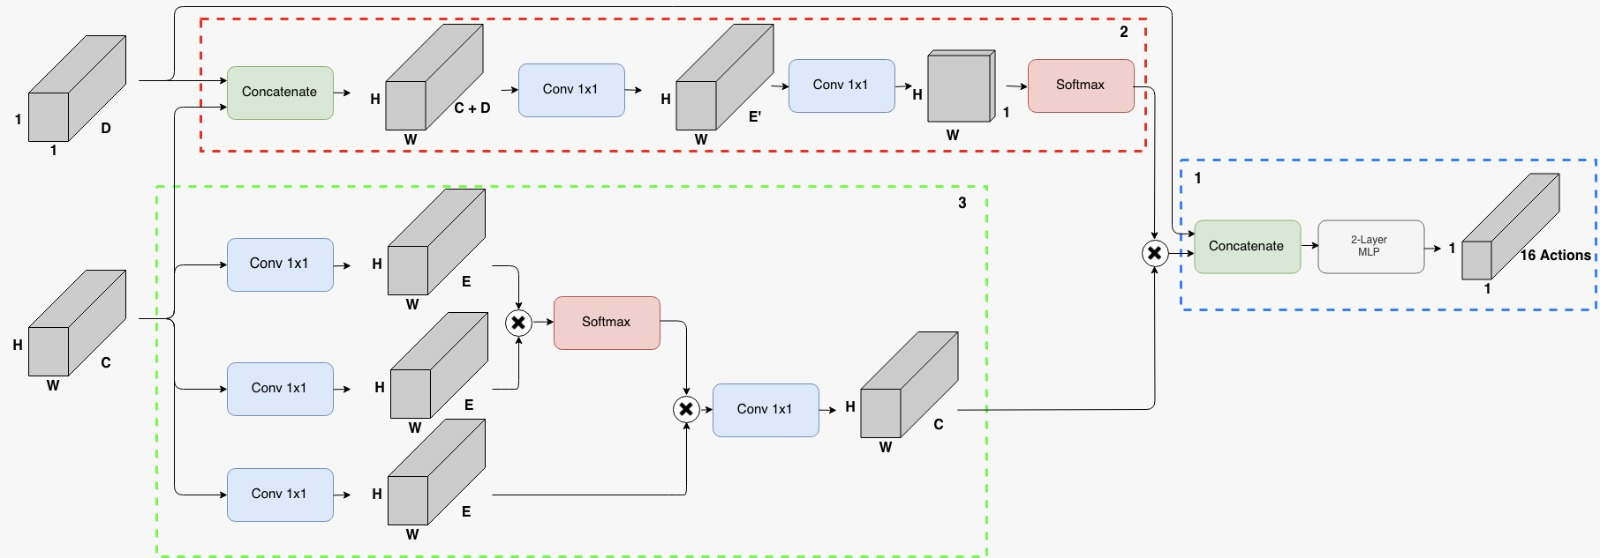
\includegraphics[width=\textwidth]{figures/model.jpg}
  \caption{The model architectures for GD-Net, GDA-Net and GDDA-Net. The green box 1 represents the fusion process of image feature and goal feature. The green box 2 is the goal-driven attention, which weights image features by learning image region-goal relation network. The green box 3 is the non-local block reasoning the image region relations.}
\end{figure*}


\section{End-to-end Visual Crowd Navigation}
In this section, we first formulate the problem of end-to-end visual crowd navigation. Later, we propose  three architectures for visual navigation taking inspiration from the 2D coordinate navigation frameworks.
 
\subsection{Problem Formulation}
In this work, we study the goal-driven visual navigation in context of crowded scenes, where an autonomous agent, given the observation $O$ and goal information $G$, needs to navigate safely and time-efficiently towards the goal.  Crowd navigation has been a challenging task due to the presence of interactions among humans in a  partially observable environment. 

Previous works \cite{helbing_social_1995, alahi_social_2016, chen_crowd-robot_2018} have studied crowd navigation by modelling the interaction between humans in 2D world coordinates. We extend the concept of human-human or human-robot interaction in 2D coordinates to region-based relation reasoning in image space, where the region can be of arbitrary size and contains enough semantic information for the agent to make decisions. There are multiple advantages of using visual observations for end-to-end learning. Firstly, instead of constraining relation modelling only to 2D coordinates of humans, we can leverage visual information from human poses or the static background environment. Second, the end-to-end learning greatly reduces the computation cost and promotes sharing of resources, capturing the interactions, by avoiding execution of a pipeline. To the best of our knowledge, this is the first work to study end-to-end learning from raw visionary input to action for the purpose of crowd navigation. 

Several factors affecting the decision-making in 2D world coordinates. The most important factor is the goal followed by the interaction with other humans, which is also referred to as repulsive effects in \cite{helbing_social_1995}, and human-human interaction \cite{alahi_social_2016, chen_crowd-robot_2018}, which is more fine-grained having indirect influence on the autonomous agent. Taking inspiration from these concepts, we propose three different models below which account for each of these factors respectively. 

% We hypothesize that to learn a good visual representation for goal-driven tasks, the model not only needs to understand the scene but also needs to reason the potential impact other objects in the scene might have on the goal acquisition. Furthermore, the model needs to reason the object relations in the image, which have indirect impact on the goal acquisition. Based on this hypothesis, we introduce dual-attention network, which models these two types of relation jointly. 

\subsection{Architectures}
 We choose the visual observation O to be depth image of size 84 x 84. The goal G is specified by the relative position $(r, \phi)$ in polar coordinate, assuming the agent can well localize itself. The goal $G$ and observation $O$ are first processed by separate learnable functions to extract coarse-grained  goal feature $g$ and image feature $x=\{x_1, x_2, ..., x_i, ..., x_n\}$ respectively. Next we describe how these two features are fused in different ways and how they are analogous to the 2D coordinate framework.

The \textbf{Goal-driven Network (GD-Net)} directly concatenates the goal feature and image feature and feeds the resulting output into another planning network. GD-Net models the relation of goal to our observation as a whole. The agent observes an image, reasons with its goal position and outputs an action. This architecture is visualized in Figure \ref{fig:model} block a. 

The \textbf{Goal-driven Attention Network (GDA-Net)} attends to important image features with respect to the goal and computes the output feature as the sum of input the image features weighted by a goal-driven attention model. The output feature is later concatenated with the goal feature, followed with a planning network. The GDA-Net models computes a score for each image feature and the goal feature, representing the amount by which the corresponding image feature influences the goal acquisition of the autonomous agent. The goal-driven attention is defined as:

\begin{equation}
\begin{aligned}
    R =&  {1 \over C_1(x)} \sum_i h(x_i, g) p(x_i)
\end{aligned}
\end{equation}
where $R$ is the final output feature representation, $h()$ takes feature $x_i$ and goal feature $g$ as input, reasons their relation and computes a scalar value representing the correlation between each image feature and the goal. $p()$ computes the response of image feature $x_i$. The final feature representation is normalized by a factor of $C_1(x)$. The attention learning part is visualized in Figure \ref{fig:model} block b.

The \textbf{Goal-driven Dual Attention Network (GDDA-Net)}  in addition to GDA-Net, computes the response of image feature $x_i$ by attending to other image features. If each image feature represents an object or an object part  then those image features should also have certain relations. These framework essentially captures the interaction between the different regions of the image. Thus, the GDDA-Net essentially models all the three interactions used in 2D navigation framework, goal, region-goal interations and region-region interactions. Following the non-local neural network \cite{wang_non-local_2017}, we choose self-attention to model the image feature relation reasoning, where $p(x_i)$ is chosen to be the weighted sum of the features at all positions in the feature sequence $x$. The definition of $p(x_i)$ is:
\begin{equation}
    p(x_i) = {1 \over C_2(x)} \sum_j f(x_i, x_j) q(x_j)
\end{equation}
where $f()$ is also a relation function between image features $x_i$ and $x_j$. $g()$ computes a representation of input signal at index j. The response is normalized by a factor $C_2(x)$. The non-local block is visualized in Figure \ref{fig:model} block c.

Combining the goal-driven attention and region region interactions, we have the entire goal-driven dual attention network is defined as:
\begin{equation}
\begin{aligned}
    R =& {1 \over C_1(x)} \sum_i h(x_i, g) [ {1 \over C_2(x)} \sum_j f(x_i, x_j) q(x_j)]
\end{aligned}
\end{equation}

% However the third effect is a second order impact a real-world object could have on the autonomous agent, and is found to be too sparse to be captured as the study showed in \cite{chen_crowd-robot_2018}. 
In simulation environment, it's harder to model the real object interactions. Thus, its difficult to analyze the performance boost we get on including the We son-how that addireging this building block doesn't degrade the performance of the network in experiment section. 
Thus modelling the region relation may not show its superiority in simulation, but it's important to consider modelling this image region relation and it could potentially benefit from learning from real world data, e.g. by analyzing the relation between a travel guide and following tourists, the network could better predict their trajectories by treating them as a group rather than treat each person as a separate identity. 

\subsection{Instantiations}
The image features are chosen to be the spatial block feature from a convolutional neural network output feature map, which is a coarse representation of objects in real world. 

Function $h()$ is modelled by a multilayer perceptron. And for the choice of image region relation function $f()$, we choose the Embedded Gaussian as in \cite{wang_non-local_2017} which is defined as:
\begin{equation}
\begin{aligned}
    f(x_i, x_j) =& e^{\theta(x_i)^T \phi(x_j)}
\end{aligned}
\end{equation}
Here $\theta(x_i), \phi(x_j)$ are embedding functions. $q(x_j)$ computes the response for image feature $x_i$ which has the embedding as $\theta()$ and $\phi()$. We implement the embedding function as 1x1 conv layer so the input shape doesn't change. 


%%%%%%%%%%%%%%%%%%%%%%%%%%%%%%%%%%%%%%%%%%%%%%%%%%%%%%%%%%%%%%%%%%%%%%%%%%
%                Attention-based demonstrator
%%%%%%%%%%%%%%%%%%%%%%%%%%%%%%%%%%%%%%%%%%%%%%%%%%%%%%%%%%%%%%%%%%%%%%%%%%

\section{Attention Measurement}
In this section, we first introduce a new method to measure attention model quantitatively by imitating an attention-based demonstrator. Then we describe our process of collecting demonstration data from demonstrator. Finally we define two measurement metrics for quantifying the attention model.

\subsection{Attention-based Demonstrator}
Quantifying the attention has been a non-trivial task because human attention is hard to measure. There is some existing work \cite{liu_attention_2016} proposed to measure the correctness of attention in neural image captioning by collecting human annotation for attention in image captioning. However collecting human annotation is time-consuming and money-consuming, which is not desirable. 

Instead of using human annotation, we propose to use an attention-based demonstrator to generate ground truth attention scores and study the problem of visual navigation in crowded spaces with imitation learning techniques, where a learner is given expert's demonstrations and it learns by mimicking the demonstrator's behavior. The demonstration consists pairs of the observation and action the demonstrator took. In order to achieve better imitation results, the learner needs to understand the causality between observation and the action. The demonstrator is attention-based policy whose behavior is explainable via the attention scores. Given the "ground truth" attention of the demonstrator, we can then quantitatively measure how close the learned attention is to the ground truth attention.

\subsection{Demonstration Collection}
For learner to learn an effective relation reasoning network, the demonstration should have reasonable causal relationship between observation and action. We leverage on recent work on crowd navigation \cite{chen_crowd-robot_2018} with attention-based deep reinforcement learning. Their work computes the attention scores on humans, which can be used as the ground truth for measuring the learned attention. We chose their main model LM-SARL as demonstrator, which models both the robot-human interaction and preserve human-human interaction through a find-grained local map. LM-SARL takes coordinates as input, which can be retrieved from the simulator. We aligned all the rest settings with the 3D simulator except that their model doesn't have field of view(FOV) limitation, which might result collisions during the deployment. After training the demonstrator policy end-to-end, we ran it in the 3D simulator with 3000 episodes. After removing the failures caused by the limited FOV, we successfully collected 117,776 pairs of observation and actions. 

\subsection{Evaluation Metrics} \label{subsection:evaluation_metrics}
Since learned attention is computed over image space and the demonstrator attention lies in world coordinates, there is no one-to-one mapping between the image region and the x,y coordinates, thus we defined two new evaluation metrics to . The first metric defines the distance between the  the demonstrator's attention and learner's attention as the difference between their highest attention directions, which is defined below:
    
\begin{equation}
\begin{aligned}
    e =& |\alpha_d - \alpha_l| \\ 
    \alpha_d =& arctan(h_y^i/h_x^i) \\
    \alpha_l =& (j / W - 0.5) * FOV + O
\end{aligned}
\end{equation}
where $\alpha_d$ is the attention direction of demonstration and $\alpha_l$ is the attention direction of the learner.
$i$ is the human who gets most attention score from demonstrator and $h_x$, $h_y$ is their x, y coordinates. $j$ is the horizontal index of the max attention value, $W$ is the width of the feature map and $O$ is the orientation of the agent. 

The second metric defines success as: the angle between two attending directions less than certain threshold values and thus compute a success rate over $n$ trials.

As for non-attention based method, i.e. GD-Net, we compute the "attention" score of one image region as the mean values over its saliency map region. The saliency map of an input image can be computed with a single back-propagation pass as proposed in \cite{simonyan_deep_2013}.


\subsection{Simulator}
To train and evaluate our model, we require a framework for perceiving surrounding humans and performing actions in the environment. And for this purpose, we built a 3D environment where humans are simulated to walk around. This simulator is based on Unreal Engine 4 to simulate human appearance, dynamics. And it uses AirSim \cite{airsim2017fsr} to retrieve depth image and interact with the environment. Collision is detected based on physical contact. Both the simulator and collected demonstration data will be released to public.


%%%%%%%%%%%%%%%%%%%%%%%%%%%%%%%%%%%%%%%%%%%%%%%%%%%%%%%%%%%%%%%%%%%%%%%%%%
%                         Experiments
%%%%%%%%%%%%%%%%%%%%%%%%%%%%%%%%%%%%%%%%%%%%%%%%%%%%%%%%%%%%%%%%%%%%%%%%%%


\section{Experiments}
To study the learning ability of the three different architectures in the visual crowd navigation task, first we compare them on collected demonstration data in supervised learning way. We then test the trained model in the simulation environment and report the performance. Finally, we quantitatively measure the distance of our learned attention to demonstrator's ground truth attention. 

\subsection{Implementation Details}
To enable the learned model better generalize to real world and bridge sim-to-real, we chose the visual observation to be depth image of size 84 x 84. The goal is specified by the relative position $(r, \phi)$ in polar coordinate, assuming the agent can well localize itself. The action space consists of 15 actions with 2 velocities evenly exponentially sampled between $(0, 1m/s]$ and 7 rotation angles evenly sampled between $[-60\degree, 60\degree]$ and one action of zero velocity and zero rotation. The autonomous agent can only observe the environment partially with a FOV of 120 degrees. The depth image is fed through convolutional layers to extract the feature maps and feature sequence consists of the spatial features Since the observation is in low resolution, the base network has three convolutional layers with 32, 64, 64 output feature channels respectively. the goal-driven attention is a two-layer perceptron with the hidden state of size 128. The embedding functions $\theta, \phi, g$ learns an embedding in 32 dimension space. After the goal feature and the image feature are concatenated, we use a three-layer perceptron to process the information, and the final output is the action class. We trained all the network with batch size 128 and learning rate 0.001 and we used Adam \cite{} optimizer.

For the simulation setup, the autonomous agent is positioned in (0, 0) with goal position (6m, 0) in the world coordinate. Humans are randomly positioned on the square of width 15m with center at (3m, 0) and randomly positioned goals. Humans are controlled by ORCA \cite{orca}, a reactive method, to guarantee collision-free with other humans. To fairly compare all the methods, simulated humans don't react to the presence of the agent. So the agent only needs to reason the perceived humans' potential influence on other humans and its goal acquisition.

\subsection{Supervised Learning on Demonstration Data}
The demonstration data consist of 117,776 pairs of image observation and action, which are divided into train, val and test in the ratio of 7:1:2. We train all models on training set and test them on the held-out validation set. The final test loss and accuracy is evaluated with the best model on validation set. 

Table \ref{tb:classification_results} shows the classification results on the collected demonstration data. The result shows that all three models can learn to predict action solely by observing the demonstrator actions. And also GDA-Net is better than GD-Net by 2\% test accuracy because GDA-Net can reason the relation between image region and aggregate them in a smarter way. The performance of GDDA-Net and GDA-Net is almost the same. The reason is probably the mutual interaction between humans are sparse and has minor indirect influence on the agent. 

\begin{table} \label{tb:classification_results}
\begin{center}
\begin{tabular}{|l|c|c|c|}
\hline
Methods & Test Loss & Test Acc. \\
\hline
GD-Net   & 1.447 & 0.508 \\
GDA-Net  & 1.407 & \textbf{0.520} \\
GDDA-Net & \textbf{1.391} & \textbf{0.520} \\
\hline
\end{tabular}
\end{center}
\caption{Test loss and accuracy with the best models selected on a held-out validation set.}
\end{table}

% Figure \ref{fig:classification_curve} shows the training loss and validation loss
% \vspace{3cm}


% \begin{figure}[tb]\label{fig:classification_curve}
%   \centering
%   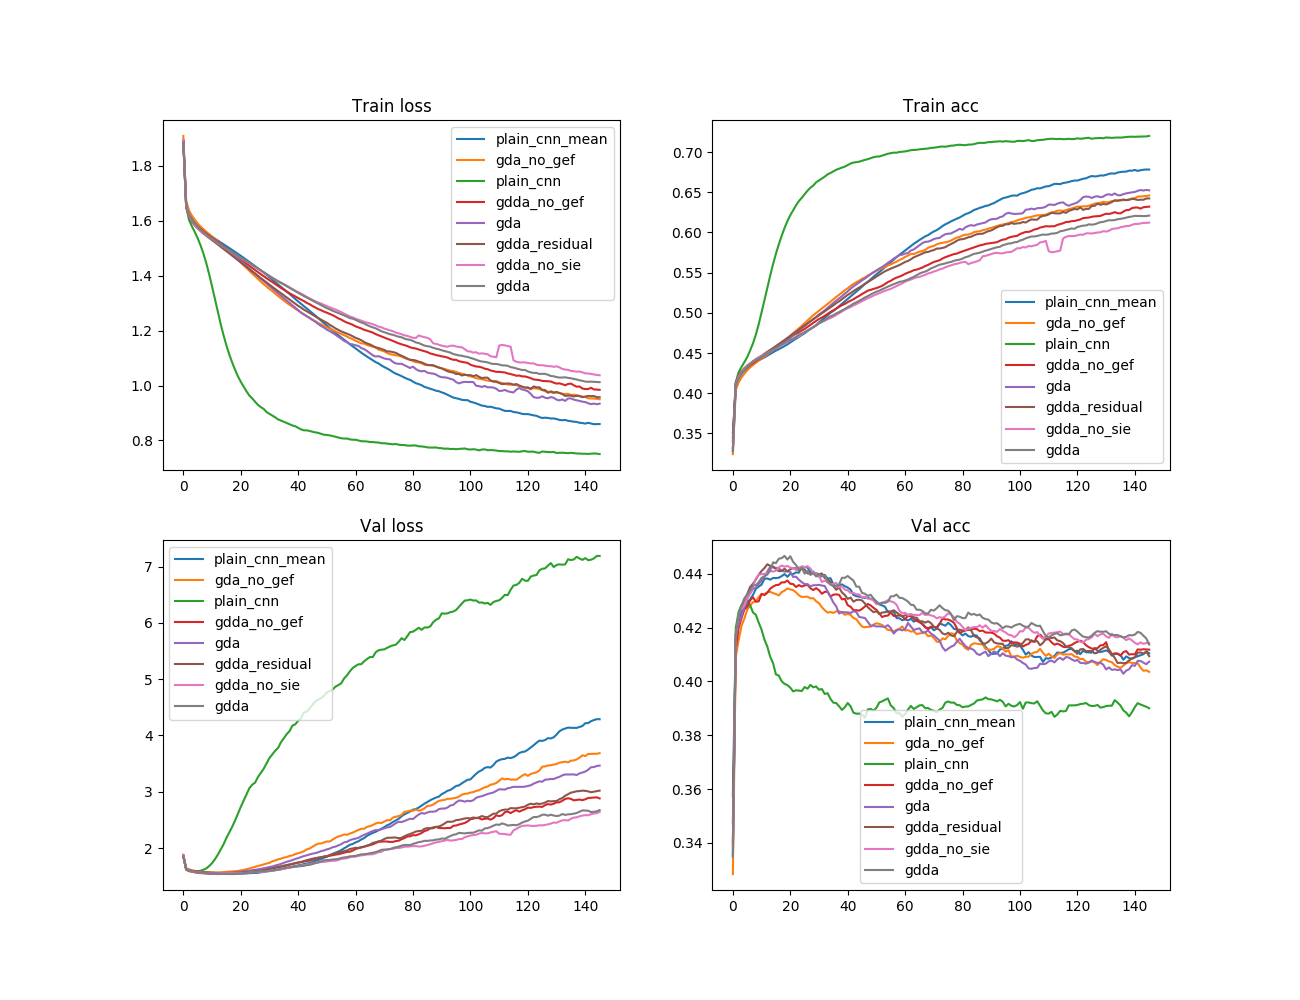
\includegraphics[width=0.48\textwidth]{figures/classification_curve.png}
%   \caption{Self-attention visualization. }
%   \label{fig:pooling}
% \end{figure}

\subsection{Test on Simulation Environment}
To further evaluate the performance of different models, we tested agent with different networks on the simulation environment with 500 test cases. We use common metrics, e.g. success rate, collision rate, timeout rate, time and etc. in crowd navigation tasks to evaluate the performance \cite{everett_motion_2018, chen_crowd-robot_2018}. To handle the the distributional drift, we added some random noise in the demonstrator's behavior when collecting the demonstration data, which eases the distributional drift problem in imitation learning \cite{}.

Table \ref{tb:simulation_results} compares the performance of different models in the simulation environment of 8 humans. Compare our attention-based with the non-attention GD-Net, we can observe the success rate increased by 3 percent. Compared with the demonstrator, there is a 17 \% drop in the success rate, which is caused by the misalignment between the demonstrator and learner setting. The demonstrator not only takes the explicit information as input, i.e. position, velocity, radius, but also these information are obtained by retrieving the ground truth. 

\begin{table} \label{tb:simulation_results}
\begin{center}
\begin{tabular}{|l|c|c|c|c|c|}
\hline
Methods & Success & Collision & Overtime & Time \\
\hline
Demonstrator    & 0.80 & 0.18 & 0.02 & 7.35  \\
\hline
GD-Net          & 0.60 & 0.40 & \textbf{0.00} & 5.97  \\
GDA-Net         & \textbf{0.63} & \textbf{0.36} & 0.01 & 6.47 \\
GDDA-Net        & \textbf{0.63} & 0.37 & \textbf{0.00} & \textbf{5.85} \\
\hline
\end{tabular}
\end{center}
\caption{Comparison of the performance between different models and the demonstrator in 500 unseen simulation scenarios. The time is only averaged over successful experiences. If the running time of one scenario is longer than certain length, then this episode is counted as over time. In this case, it's 50 seconds in game time.}
\end{table}

Figure \ref{fig:attention_visualization} shows attention visualization in one observed frame along with the top-down view ground truth attention of the demonstrator. From the right image, we find the demonstrator assign the highest attention score to the human 1 instead of closest human 3, which makes sense because human 3 is walking away from the autonomous agent and human 1 is walking toward him. From the left depth image, we can see the learner also assign the highest attention to human 1 instead of human 3. The other humans who are farther are only assigned very little attention.


\begin{figure}[tb]\label{fig:attention_visualization}
  \centering
  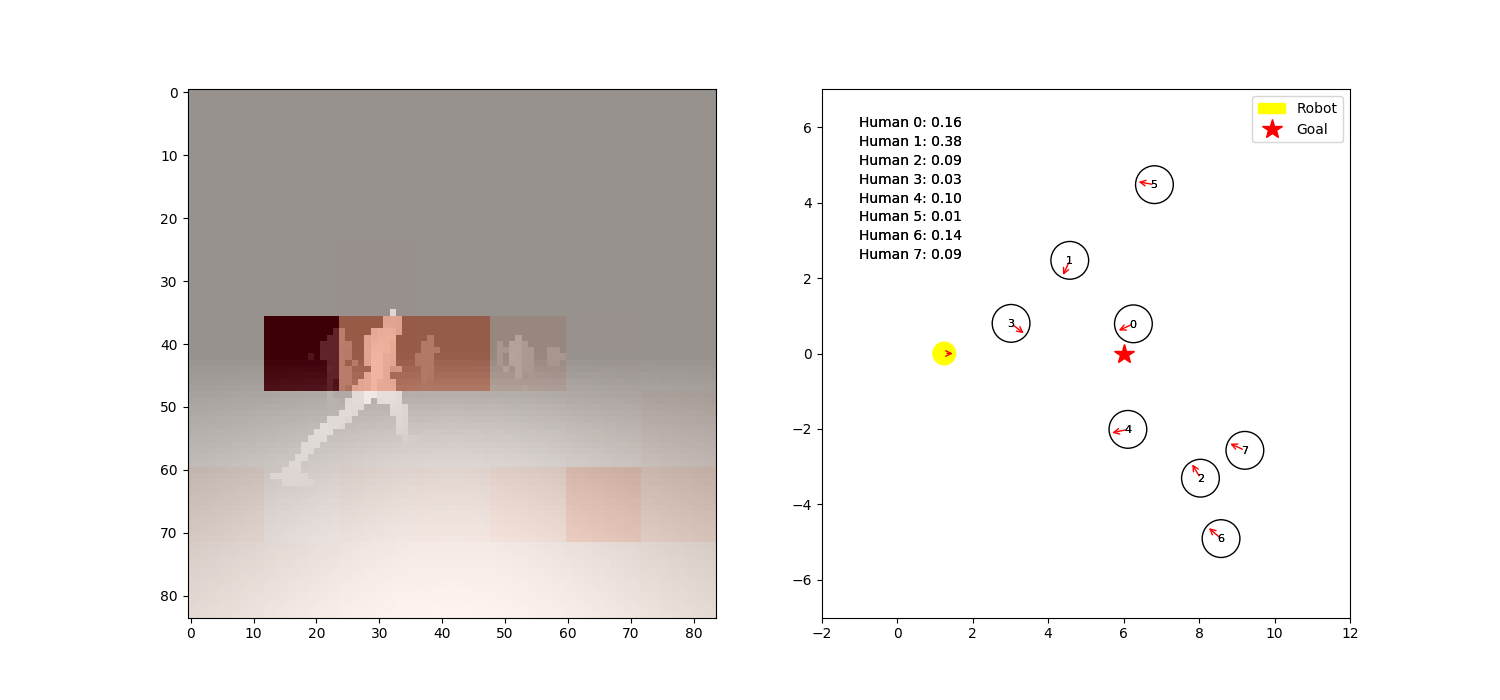
\includegraphics[width=0.48\textwidth]{figures/attention_8h_3.png}
  \caption{Attention visualization case 1. Left figure shows the depth image perceived by the agent and visualized with attention map. The redder a block is, the more attention the agents pays to that block. Right is the top-down view of the agent and its surrounding humans indicating the ground truth attention. The agent has a FOV of 120 degrees and the left corner scores show the attention weight it assigns to each human.}
\end{figure}

\subsection{Attention Measurement}
To further investigate whether attention really works, we evaluate the learned attention with the ground truth attention provided by the demonstrator using the metrics defined in \ref{subsection:evaluation_metrics}. Since all the models don't necessarily predict the same action, to avoid the difference of observation caused by the accumulated movement error. We let demonstrator perform the action and at each step, we retrieve visual observation from the simulator and run other models to produce the attention map.

Table \ref{tb:attention_diff} reports the performance of different models under the defined metric. Also we report the performance of a random policy that picks a random direction to attend. Compared to random policy, our networks attend more accurately. Compare GDA-Net and GDDA-Net with the GD-Net, which is non-attention based, we can still observe on average 0.06 radian reduction. The reason for that is the goal-driven attention not just detects the salient object, but actually reasons how each region could affect its goal acquisition, which also show the learner learns to recover the demonstrator attention by just reasoning the causality between observation and action.

\begin{table} \label{tb:attention_diff}
\begin{center}
\begin{tabular}{|l|c|c|}
\hline
Methods & Angle & Accuracy\\
\hline
Random                  & 0.6857 & 0.1429 \\
\hline
GD-Net(Saliency)        & 0.6273 & 0.3052 \\
GDA-Net                 & 0.5685 & 0.2836 \\
GDDA-Net                & \textbf{0.5648} & \textbf{0.3521} \\
\hline
\end{tabular}
\end{center}
\caption{Comparison of three architectures and a random policy on the distance to the ground truth. The first column measures the angle between demonstrator's and learner' attending direction. The second column measures the success rate of the learner's attention. These results are }
\end{table}

Figure \ref{fig:attention_comparison} From the top-down view, we know the agent GDDA-Net and GDA-Net is able to find the important human although he's a bit far and blurry. However the GD-Net didn't even capture that human because we can see the corresponding blocks are assigned little weights. 

\begin{figure}[tb]\label{fig:attention_comparison}
  \centering
  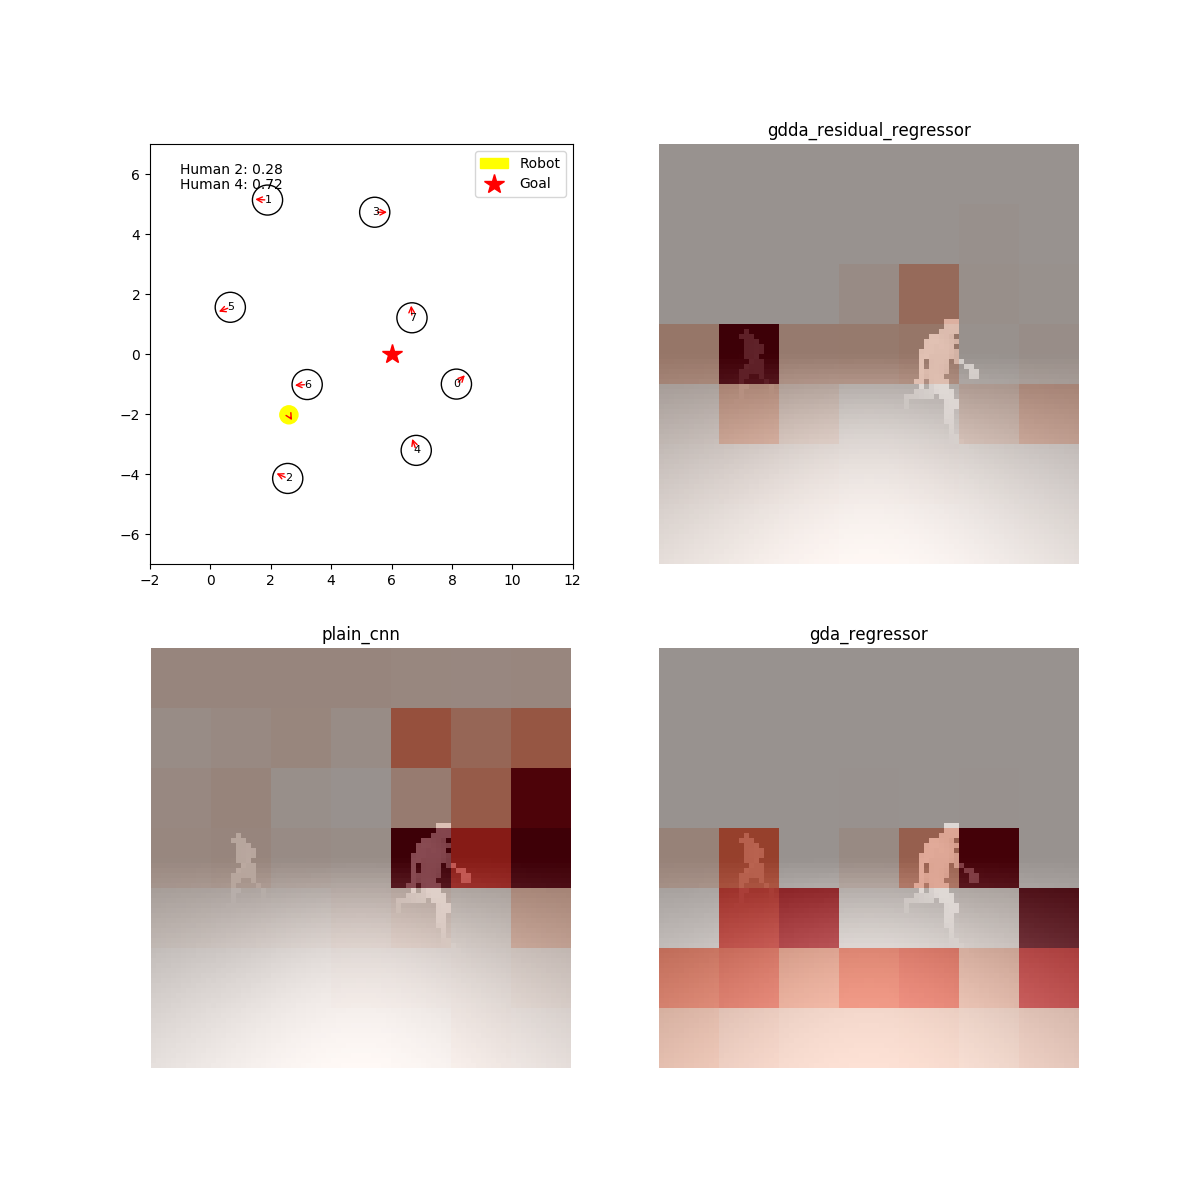
\includegraphics[width=0.48\textwidth]{figures/attention_comparison.png}
  \caption{Attention comparison given the same visual observation. Top-left is the top-down view of human and agent position, velocity. And the top-left corner is attention scores given by attention-based demonstrator, from where we can see the demonstrator assigns more weights to agent 4. And from the rest three attention visualization, we can see the GD-Net missed the important person, the other two network captured the human but GDA-Net assigns lower weight to him compared to the one closer.}
\end{figure}

\section{Conclusion}

% \begin{figure*}
% \begin{center}
% \fbox{\rule{0pt}{2in} \rule{.9\linewidth}{0pt}}
% \end{center}
%   \caption{Example of a short caption, which should be centered.}
% \label{fig:short}
% \end{figure*}


{\small
\bibliographystyle{ieee}
\bibliography{vita-visual-nav}
}

\end{document}
